\section{Aceleración}
Cotidianamente podemos observar que los automóviles de las calles cambian su velocidad: frenan cuando llegan a una esquina (disminuyen su velocidad), aceleran luego de observar que es seguro cruzar la calle (aumentan su velocidad). En términos físicos, los automóviles {\it desaceleran} (frenan) cuando llegan a la esquina y luego {\it aceleran} para cruzar la calle. Que tan rápido varía la velocidad (disminución o aumento) en un instante (o intervalo) de tiempo, es lo que entiende la física por {\bf aceleración}.

\subsection{Aceleración media}

La {\bf aceleración media }se define como la razón entre la variación de velocidad $\mathbold{\Delta v}$ y el intervalo de tiempo $\Delta t$, en que se ha producido dicha variación:

\begin{center}
\boxed{\mathbold{\bar{a}_m}=\frac{\mathbold{\Delta \bar{v}}}{\Delta t}=\frac{\mathbold{\bar{v}}-\mathbold{\bar{v}_0}}{t-t_0}}
\end{center}

en donde dicha aceleración es una {\bf magnitud vectorial} la cual tiene la misma dirección y sentido que la variación de velocidad $\mathbold{\Delta \bar{v}}$, debido a que $\Delta t > 0$. 


Las unidades con que se miden las aceleraciones surgen, al igual que las velocidades, de la misma operación que las define. Se trata de un cociente entre una velocidad ($\Delta v$) y un intervalo de tiempo ($\Delta t$). Con esta expresión: $$[a_m] = \frac{[\Delta v]}{[\Delta t]}$$
Si trabajamos en el SIMELA, la unidad derivada es: $$[a_m] =\sif{$\!\!\sif{m}{s}$}{s} =\frac{\textrm{m}}{\textrm{s}^2}$$


{\bf \color{BrickRed} {¡Cuidado!}} En la vida cotidiana la palabra {\it aceleración} está asociada con el {\it movimiento}. Sin embargo, que un cuerpo no se esté acelerando o desacelerando, {\bf no implica que no se esté moviendo}. ¡Dicho cuerpo puede estar en movimiento con velocidad constante!
\\


Veamos gráficamente un caso rectilíneo en donde un automóvil que recorre el trayecto $P_0$ - $P$, cambia desde una velocidad $\mathbold{\bar{v}_0}$ hasta una velocidad $\mathbold{\bar{v}}$ de mayor módulo en un intervalo de tiempo $\Delta t$

\begin{figure}[!h]
\centering
 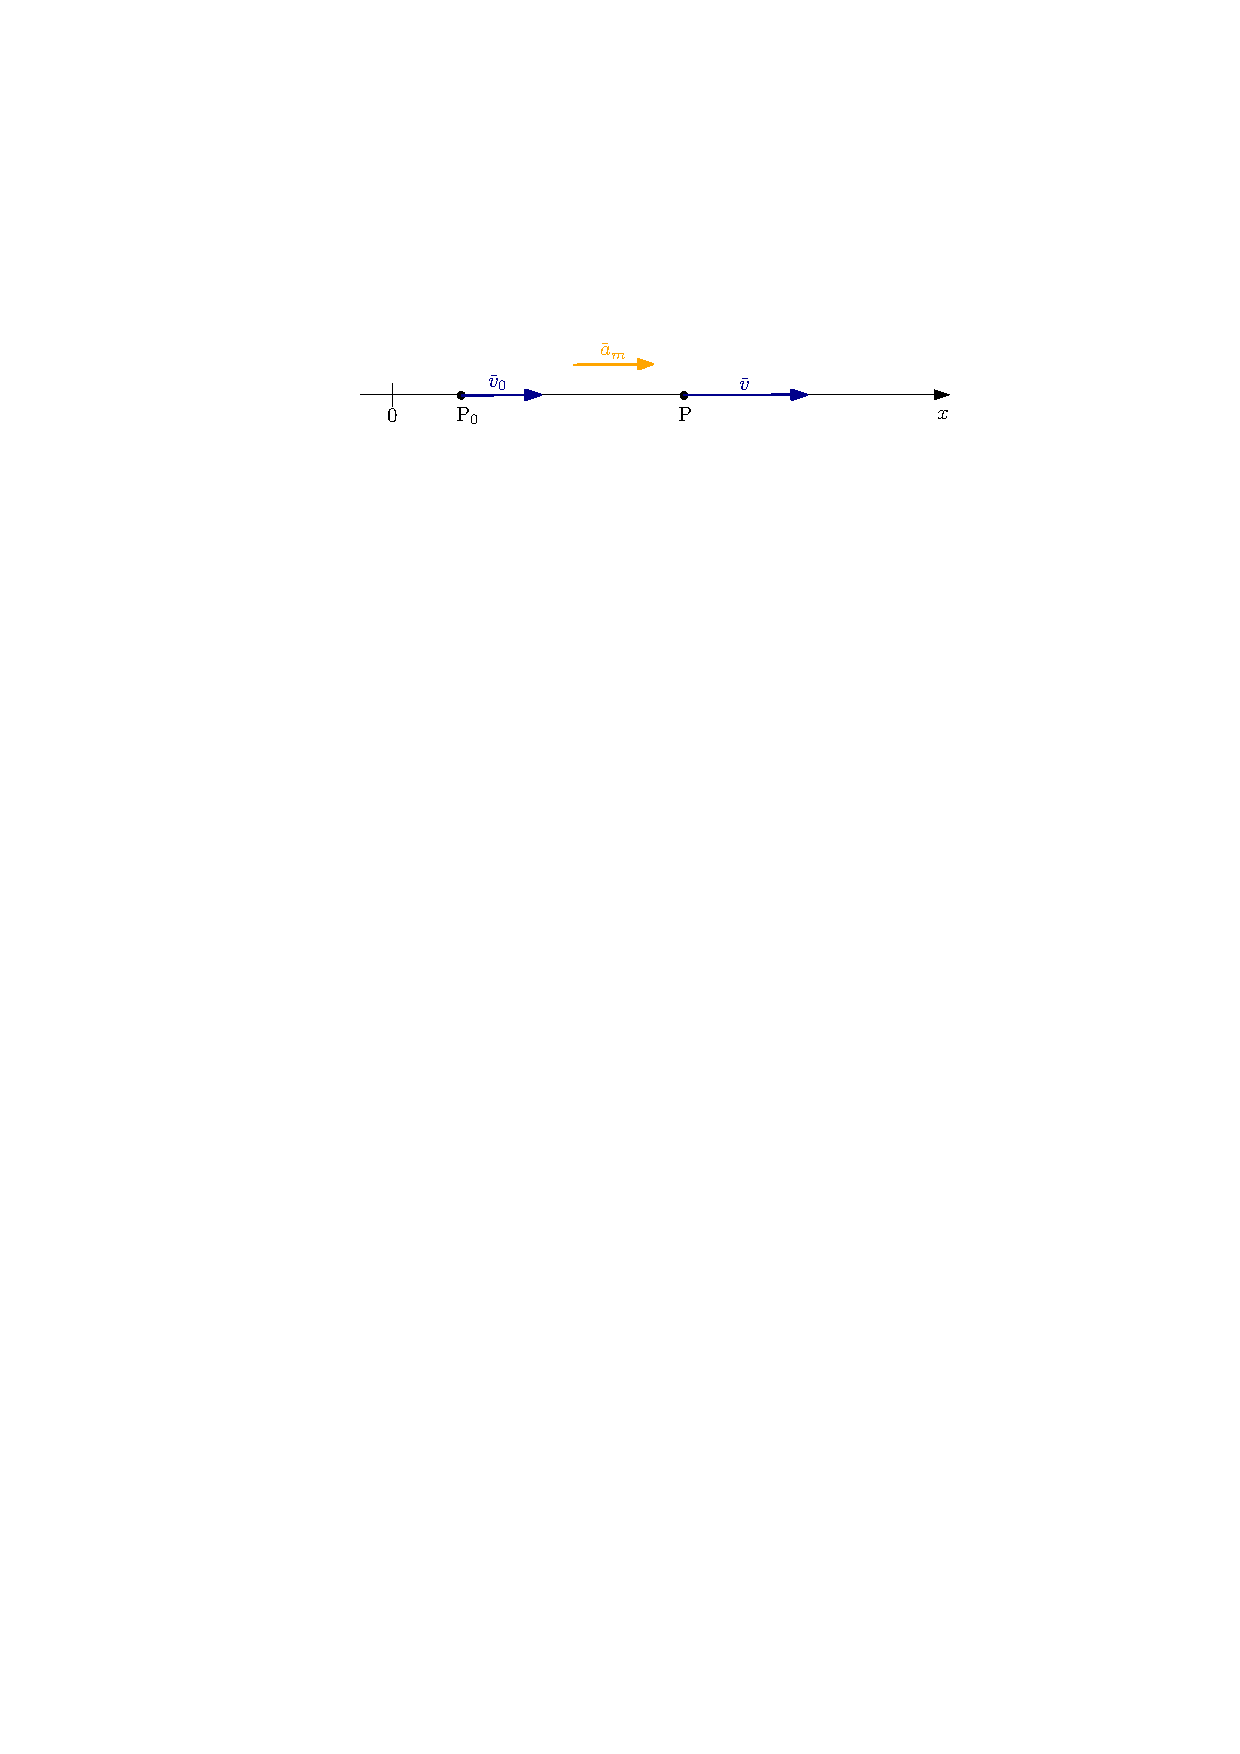
\includegraphics[width=.6\textwidth]{img/amedia.pdf}
 \caption{Aceleración media en un movimiento rectilíneo.}
\end{figure}


Como ya se dijo, la aceleración es una magnitud vectorial. Pensemos en dos automóviles que están acelerando  uniformemente por la misma ruta en sentidos opuestos a 5\,km/h$^2$ y 10\,km/h$^2$, respectivamente. Teniendo en cuenta el sistema de coordenadas estas aceleraciones resultarán de signo opuesto:



\begin{figure}[!h]
\centering
 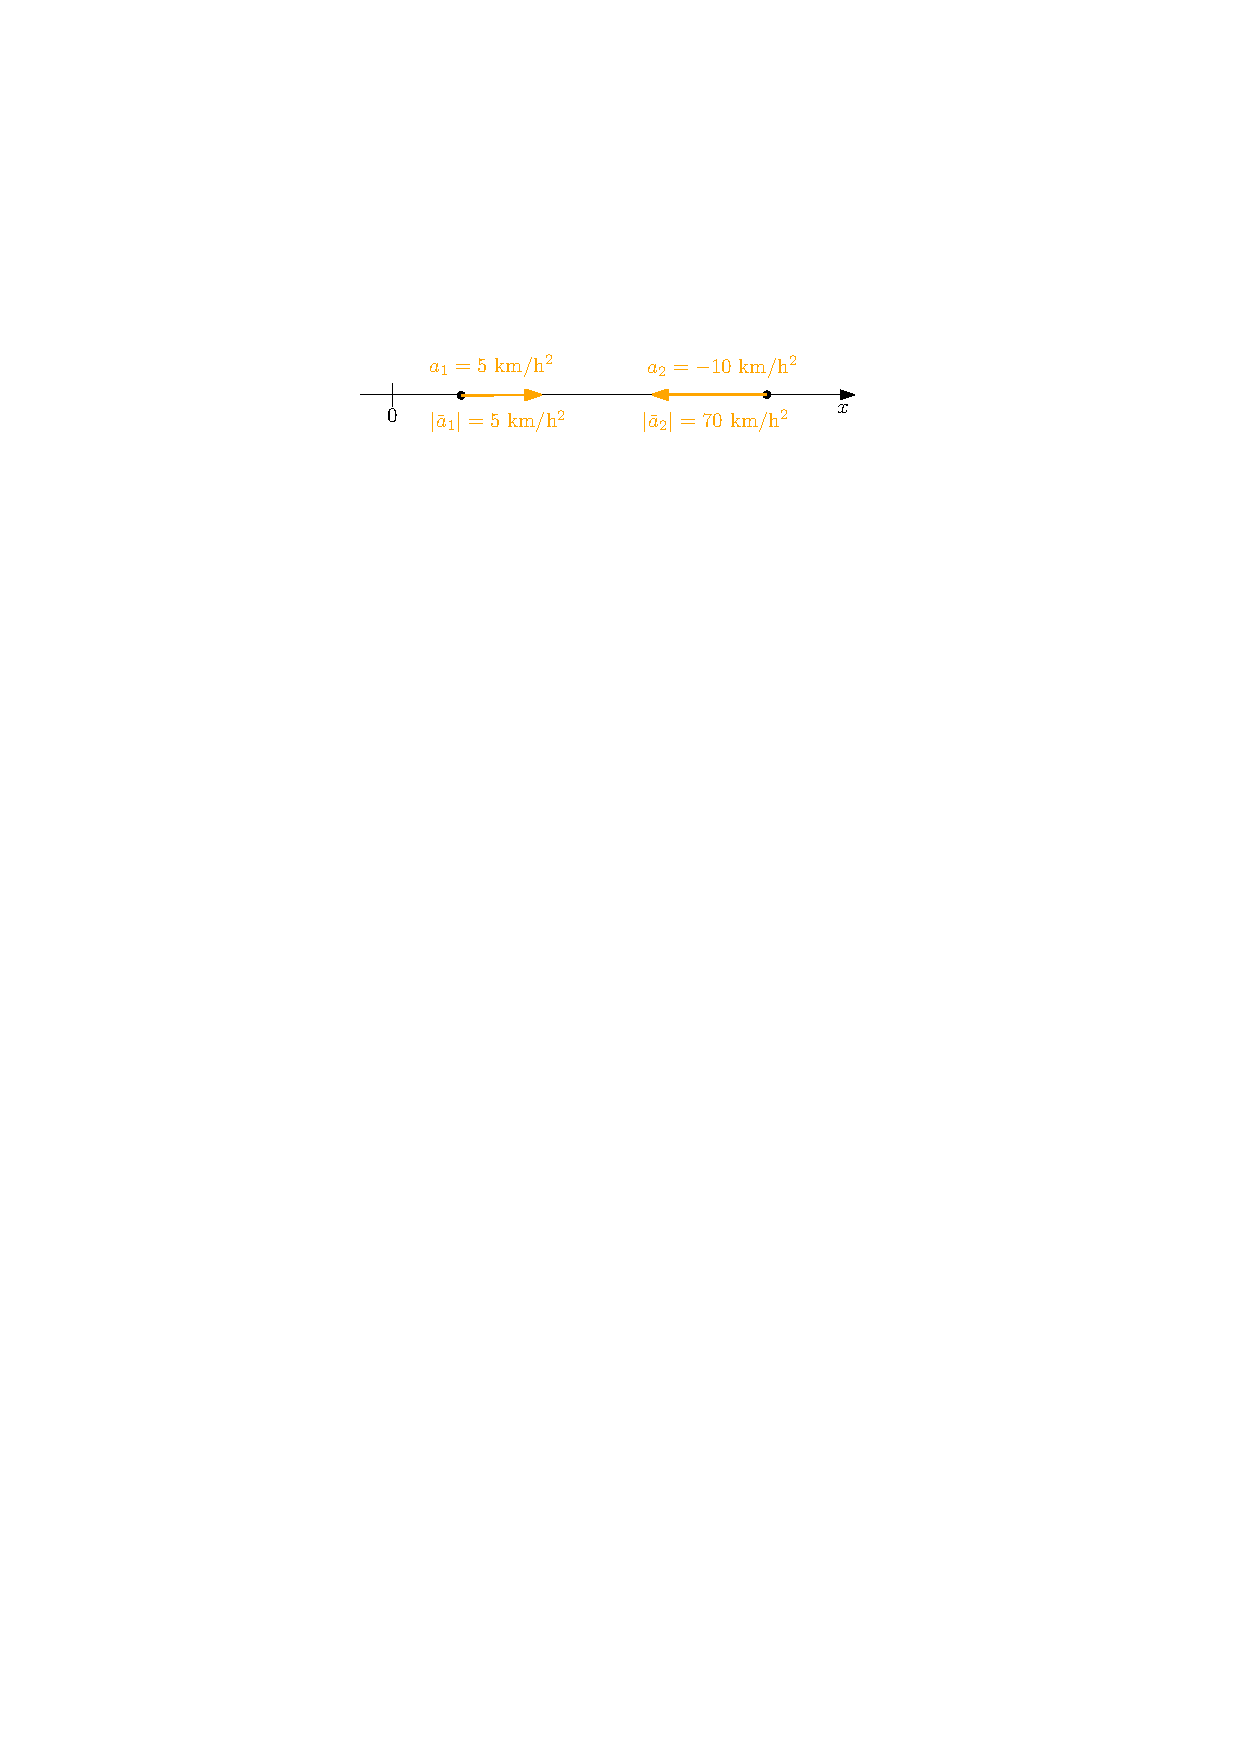
\includegraphics[width=.6\textwidth]{img/acomp1.pdf}
% \caption{Aceleración media en un movimiento rectilíneo.}
\end{figure}

El signo de la aceleración \textbf{depende del sistema de coordenadas}.


{\bf \color{BrickRed} {¡Cuidado!}} En el ejemplo anterior, al igual que acurre con la velocidad, cuando decimos ``$a_1= 5$ km/h'' o ``$a_2= -10$ km/h'', {\bf ¡nos estamos refiriendo a la componente $x$ del vector aceleración!} Debido a que el movimiento es rectilíneo, es decir que la partícula se mueve en el eje $x$, podemos utilizar esta notación. Si el movimiento fuera en un plano deberíamos escribir sus dos componentes:

\begin{figure}[h!]
\centering
 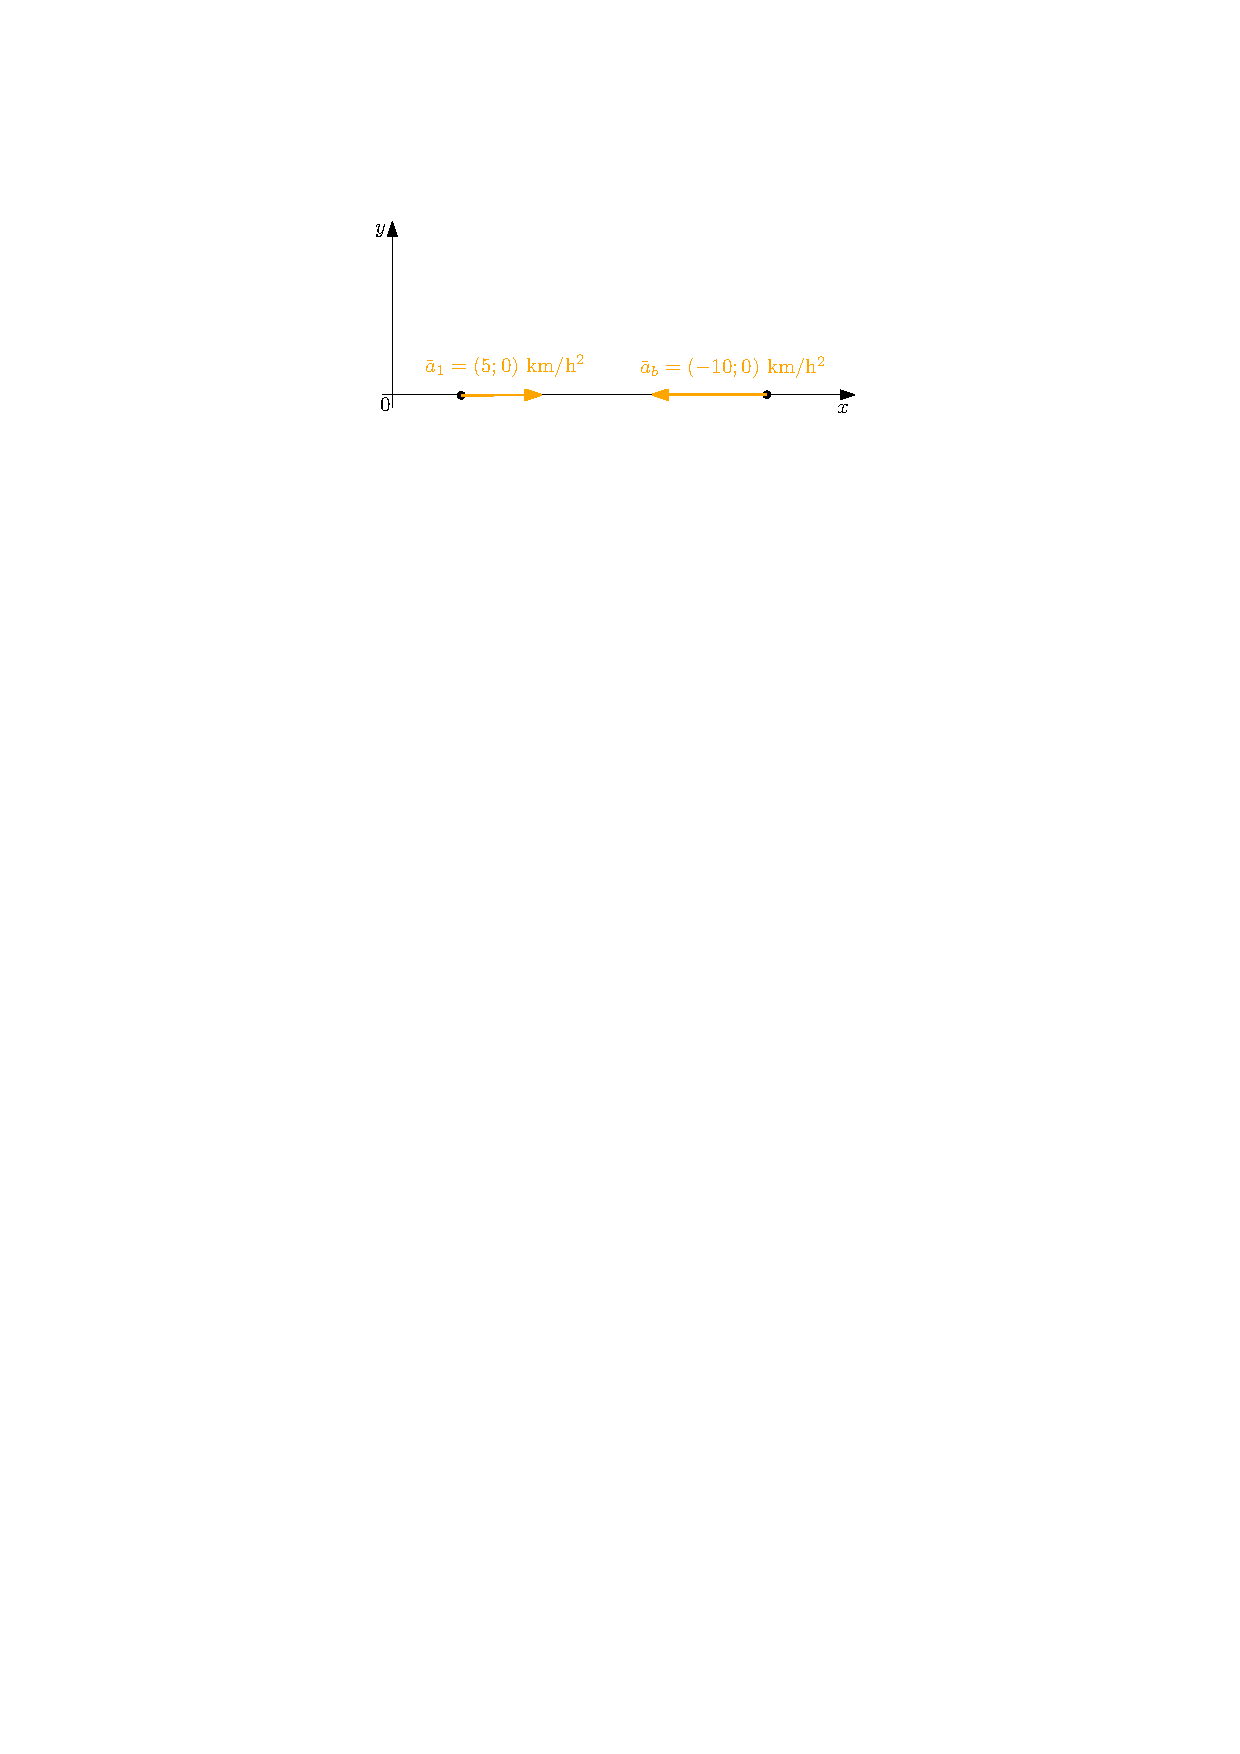
\includegraphics[width=.6\textwidth]{img/acomp2.pdf}
 % \caption{Velocidad media en un movimiento rectilíneo.}
\end{figure}



Retomando el análisis del principio de la sección, si decimos que un objeto {\it acelera} o {\it desacelera}, nos estamos refiriendo a cómo varía la rapidez, sin pensar en la dirección o el sentido de la velocidad. 

¿Cómo sabemos si una partícula está \textit{acelerando} o \textit{desacelerando}?

\info{
    Contrario a lo que se tiende a pensar, no es el signo de la aceleración por sí solo el que indica si una partícula \textit{acelera} o \textit{desacelera}.}
    
Podremos saber si un objeto está acelerando o desacelerando comparando el signo de la velocidad con el signo de la aceleración. ¿Cómo es esto? Debemos tener presente que \textbf{la aceleración nos indica cómo cambia la velocidad}, si la aceleración apunta en el mismo sentido que la velocidad, esta aumentará su módulo pero si, por el contrario, ambas apuntan en sentido opuesto, la velocidad disminuirá su módulo.

En los cuatro ejemplos de la Figura siguiente se observan las posibles combinaciones de $\mathbold{\bar{v}}$ y $\mathbold{\bar{a}}$ que podemos tener, todas para un mismo sistema de referencia.

\begin{figure}[H]
 \begin{subfigure}{0.5\textwidth}
    \centering
 	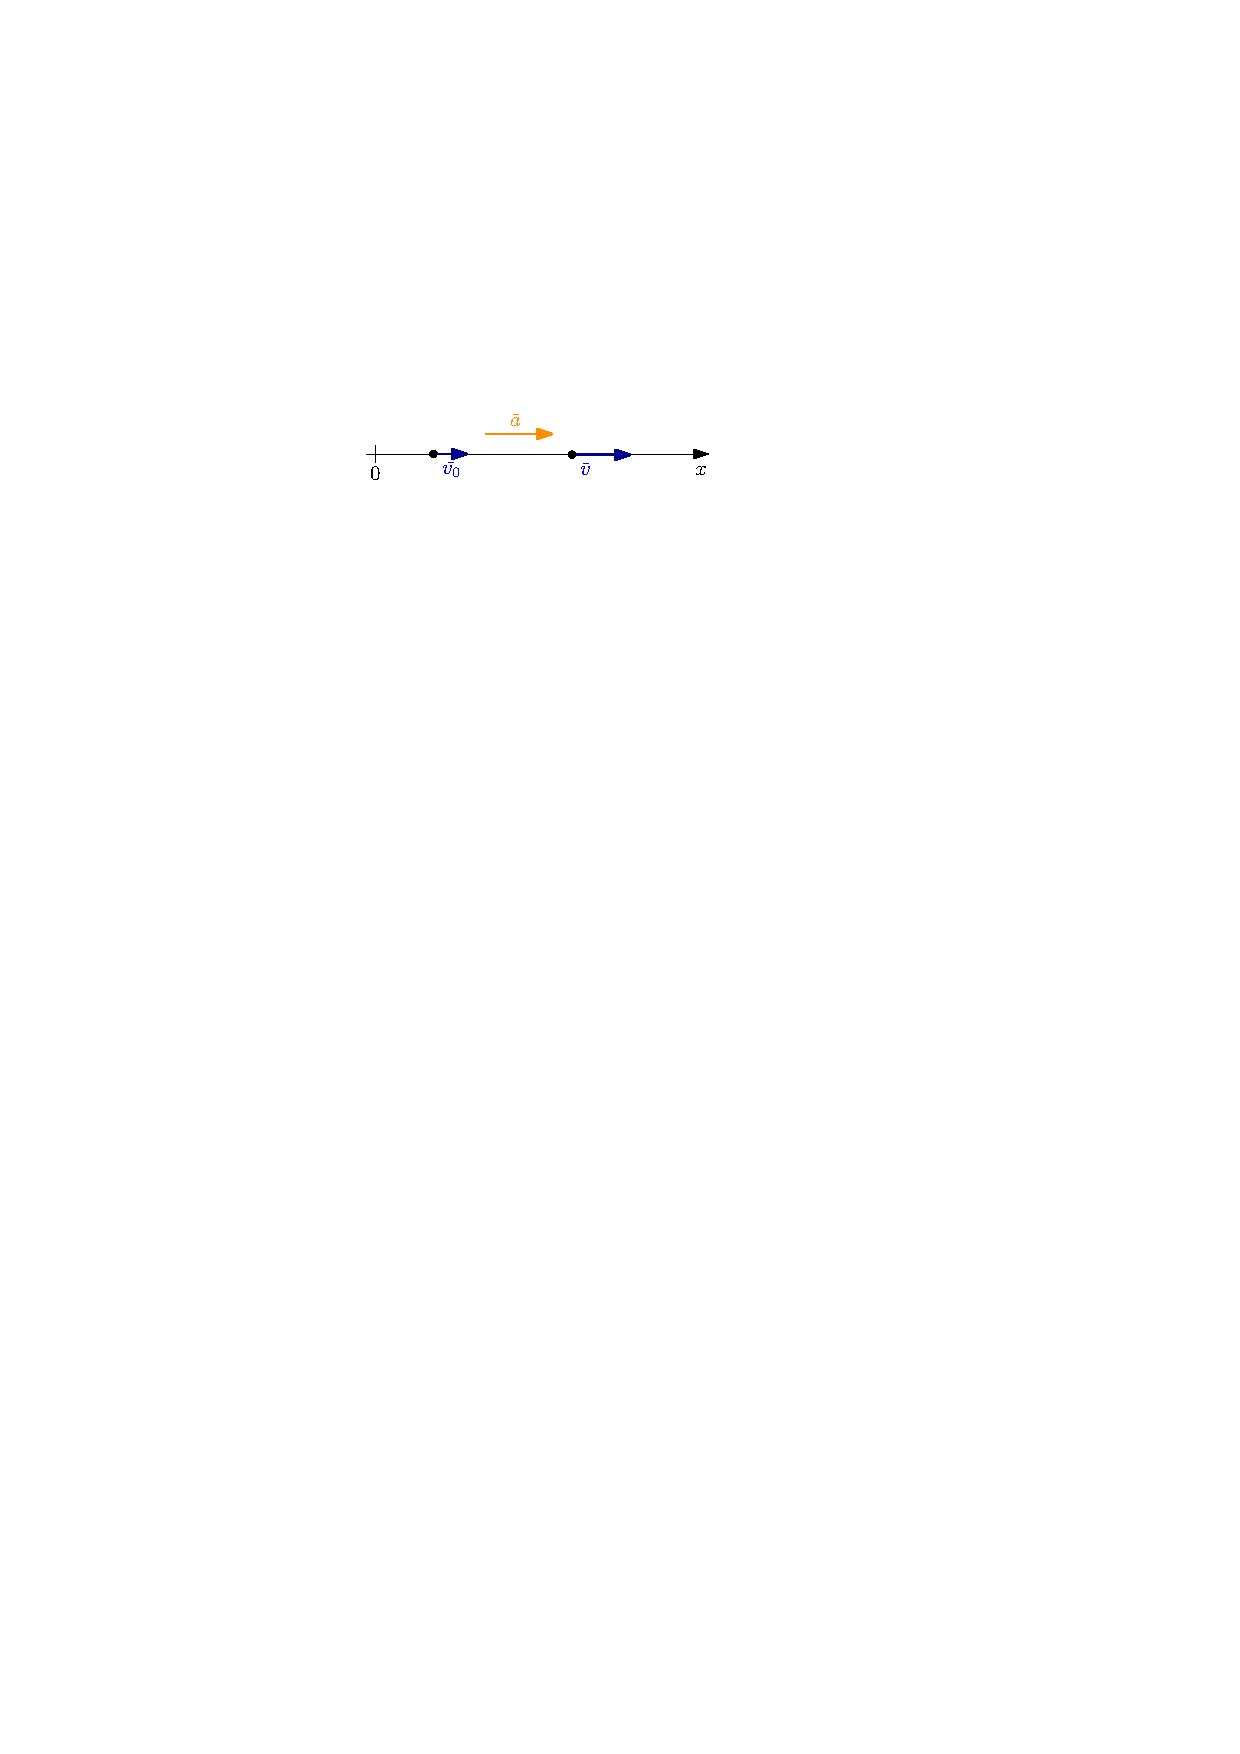
\includegraphics[width=.9\linewidth]{img/acelera1.pdf}
	\caption{$a>0$ y  \textit{acelera}}	
\end{subfigure}   
 \begin{subfigure}{0.5\textwidth}
    \centering
 	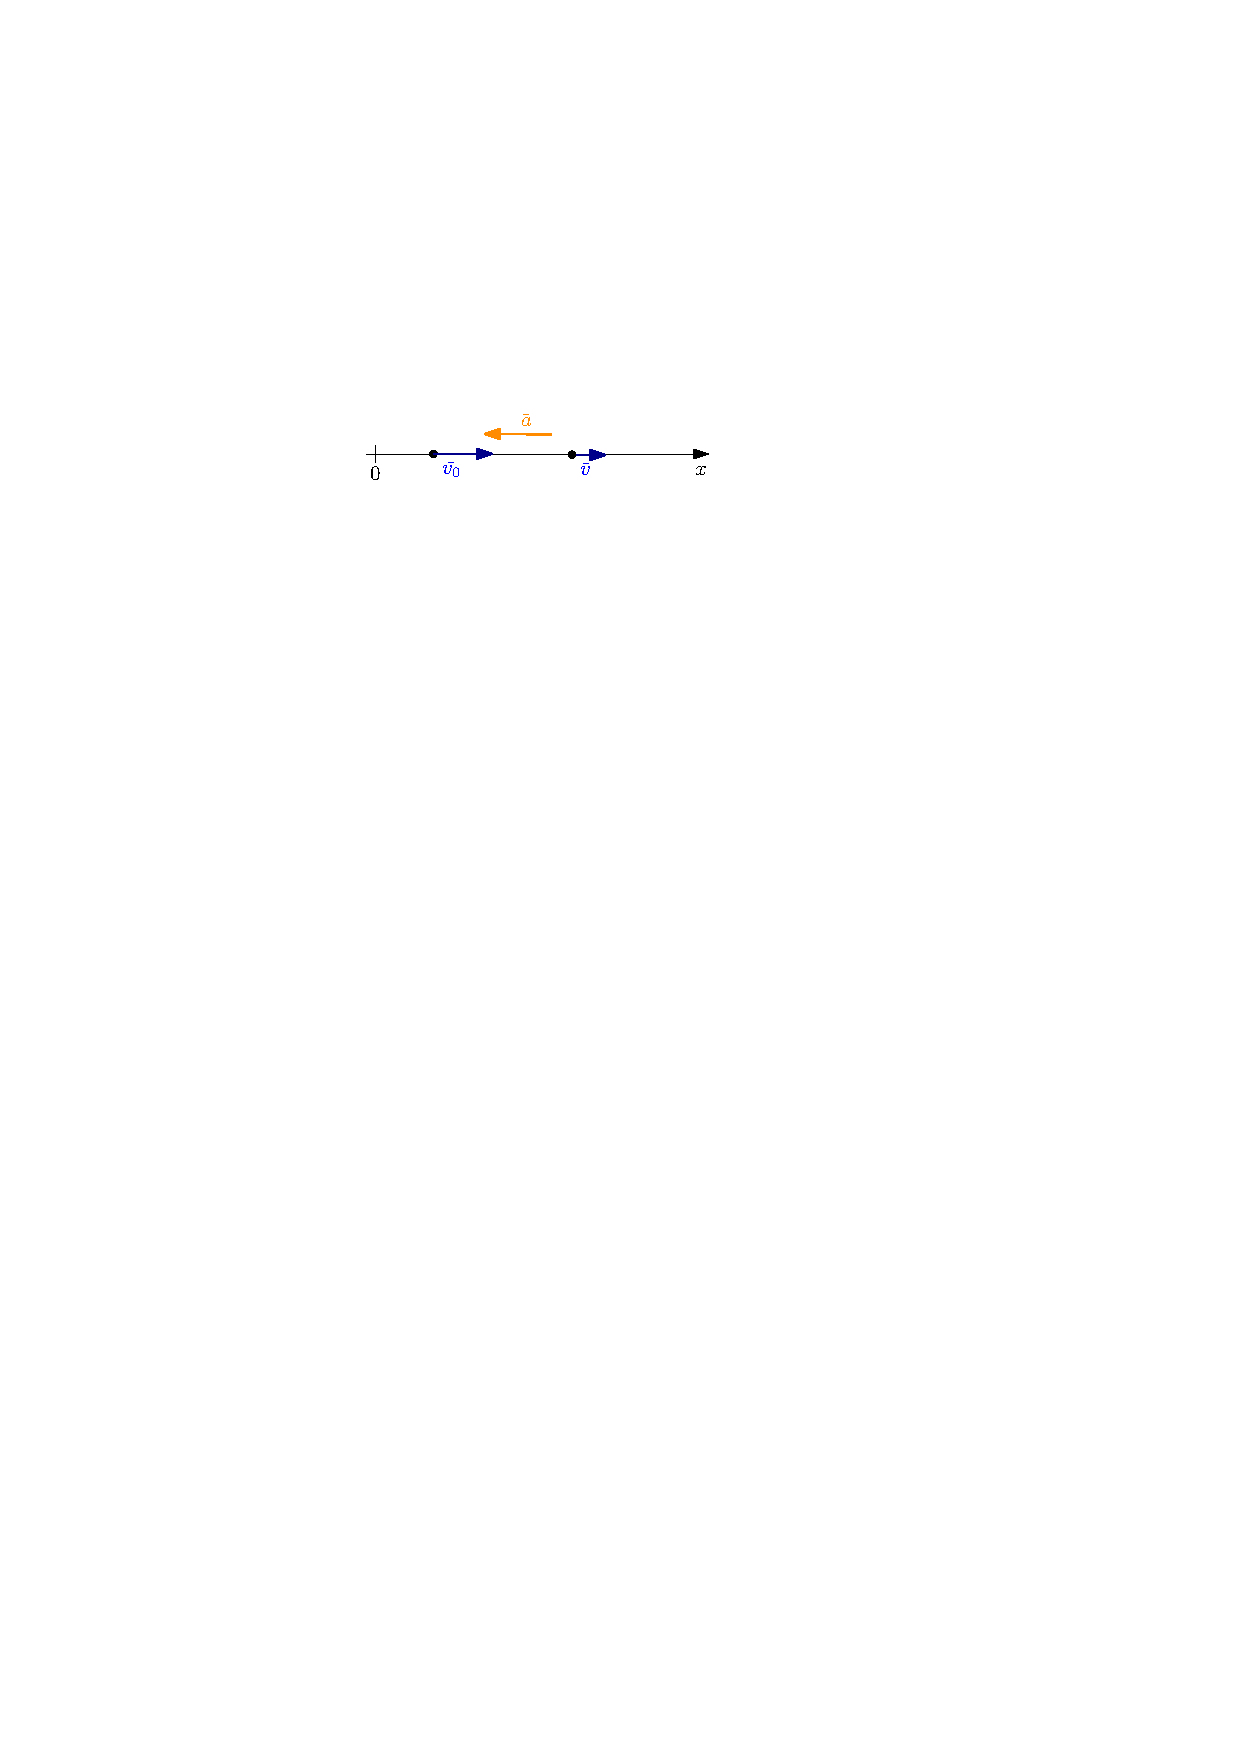
\includegraphics[width=.9\linewidth]{img/acelera2.pdf}
	\caption{$a<0$ y \textit{desacelera}}	
\end{subfigure}
 \begin{subfigure}{0.5\textwidth}
    \centering
 	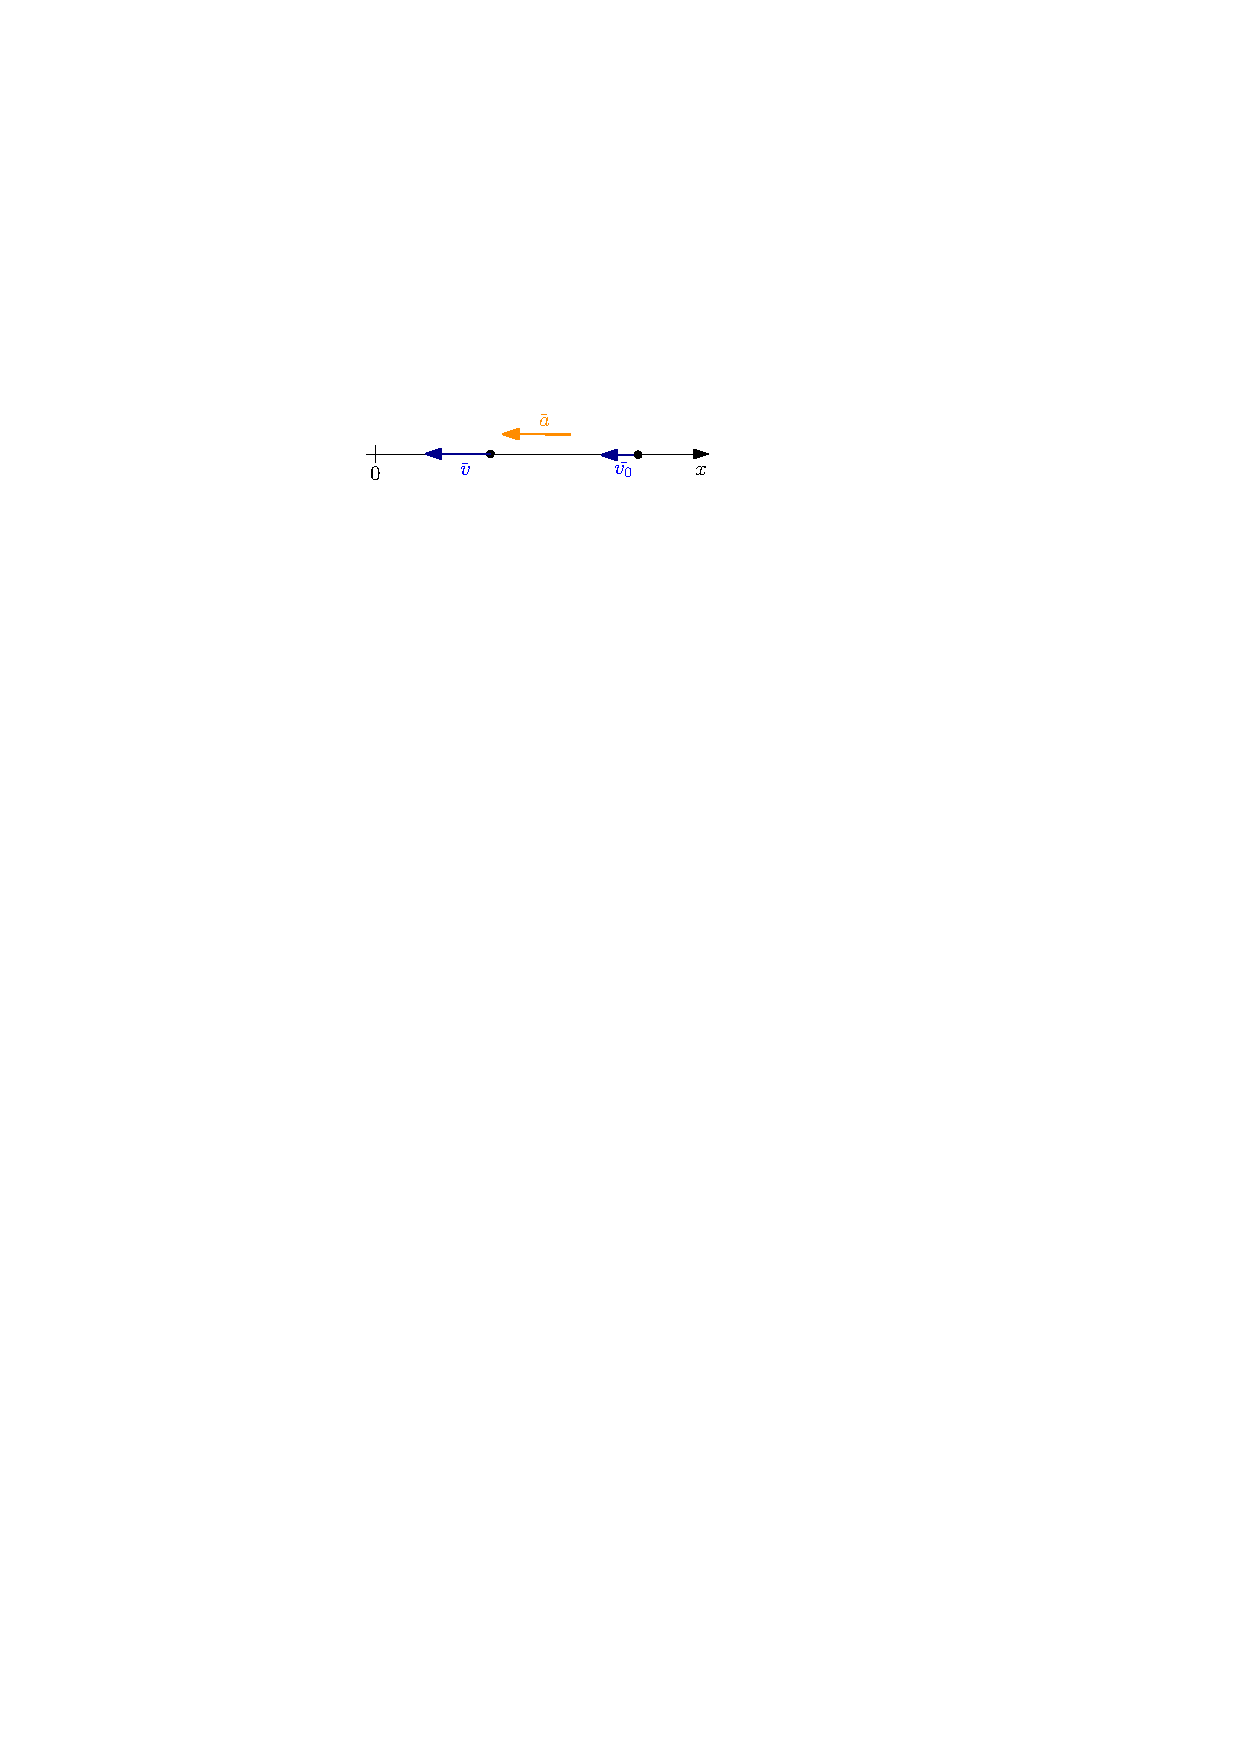
\includegraphics[width=.9\linewidth]{img/acelera3.pdf}
	\caption{$a<0$ y \textit{acelera}}	
\end{subfigure} 
 \begin{subfigure}{0.5\textwidth}
    \centering
 	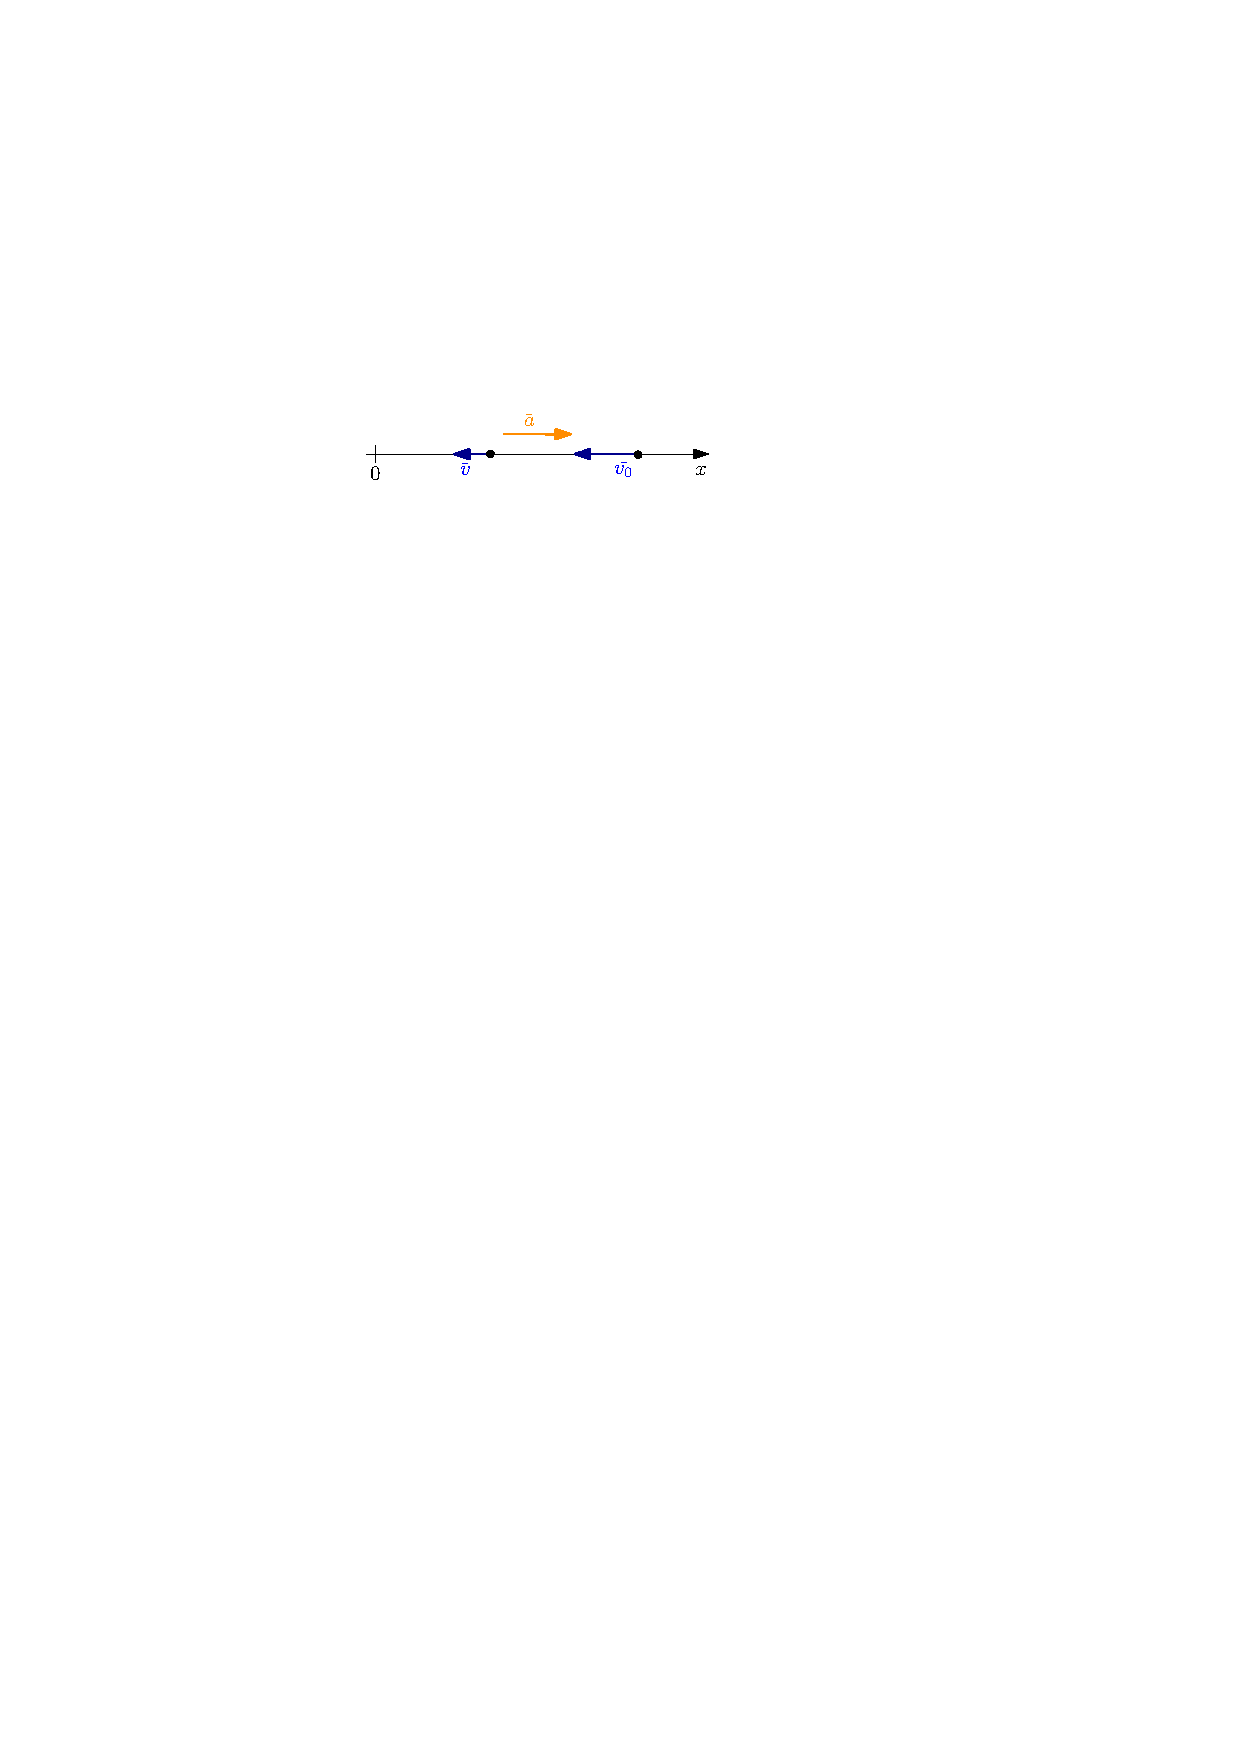
\includegraphics[width=.9\linewidth]{img/acelera4.pdf}
	\caption{$a>0$ y \textit{desacelera}}	
\end{subfigure} 
\end{figure}








\info{

Si viajamos en un automóvil que se mueve con velocidad constante, sin la posibilidad de mirar hacia afuera, nos es {\it imposible} decir que dicho automóvil está en movimiento o en reposo. En otras palabras {\bf ¡no podemos percibir la velocidad!} En cambio, si éste aumenta su velocidad (acelera), experimentamos dicho aumento al recargarnos más contra los asientos. Y si disminuye su velocidad (desacelera), nos despegamos de dichos asientos. En otras palabras {\bf ¡podemos percibir la aceleración!}}



Recordemos que la velocidad también es una magnitud vectorial. Por lo tanto un cambio en la velocidad $\mathbf{\Delta \bar{v}}$ implica que la misma puede haber cambiado su:
\begin{itemize}
\item {\bf módulo} (rapidez)
\item {\bf dirección}
\item {\bf sentido}
\end{itemize}


\begin{comprension}
¿Puede un móvil realizar un movimiento con rapidez constante aún cuando su velocidad varía?\\
{\em Ayuda: Piensa en un movimiento en el plano.}
\end{comprension}


Dado su carácter vectorial, la aceleración es entonces un concepto que contempla:

\subsubsection{Cambio en el módulo de la velocidad}

\begin{figure}[H]
\centering
 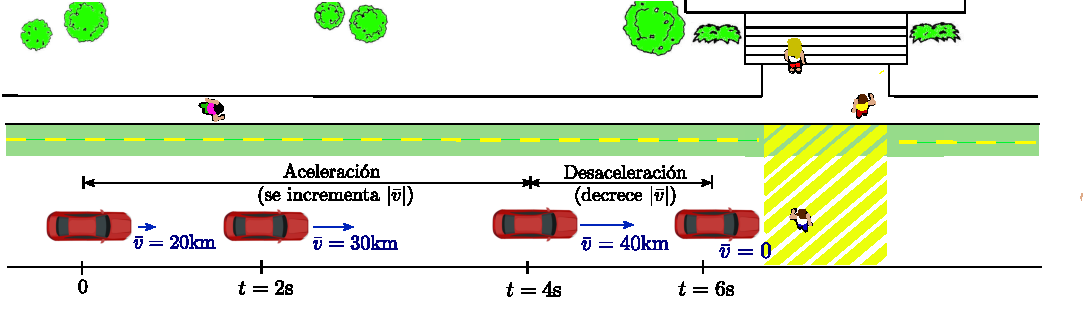
\includegraphics[width=1.1\textwidth]{img/auto1.pdf}
 \caption{Aceleración debido a la variación del módulo de la velocidad.}
\end{figure}

\subsubsection{Cambio en la dirección o el sentido de la velocidad}

\begin{figure}[H]
\centering
 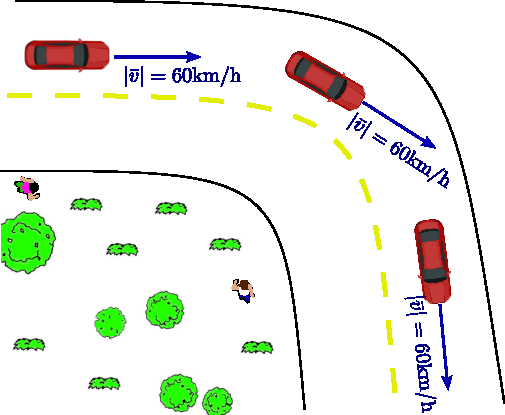
\includegraphics[width=.5\textwidth]{img/auto2.pdf}
 \caption{Aceleración debido al cambio en la dirección de la velocidad.}
\end{figure}


\subsection{Aceleración instantánea}

En algunas situaciones el valor de la aceleración media puede ser diferente en intervalos de tiempo distintos. Por este motivo es útil definir la {\bf aceleración instantánea}, como hicimos anteriormente con la velocidad instantánea:


$$\mathbold{\bar{a}}= \lim_{\Delta t \rightarrow 0} \mathbold{\bar{a}_m} = \lim_{\Delta t \rightarrow 0} \frac{\mathbold{\Delta \bar{v}}}{\Delta t}$$